\chapter{System Evaluation}
\label{ch:evaluation}

This chapter reports the quantitative results for the two artifacts. I separate the single-node and distributed results because they answer different questions. LKC-CXL-PIM asks how much decode work can be moved into one CXL-attached HBM endpoint. DisaggKV asks whether the same traffic reduction remains useful when the KV cache is distributed across endpoints. Table~\ref{tab:results_summary} gives the single-node counters that are used repeatedly in the discussion.

\begin{table}[htbp]
\centering
\caption[Summary of single-node results]{Summary of quantitative single-node results for the baseline and LKC-CXL-PIM.}
\label{tab:results_summary}
\begin{tabular}{lcccc}
\toprule
\textbf{Context Length} & \textbf{Metric} & \textbf{Baseline} & \textbf{LKC-CXL-PIM} & \textbf{Improvement} \\
\midrule
\multirow{2}{*}{8K}   & Read Latency (M Cycles) & 10.77 & 0.12 & 91.5$\times$ \\
                      & Row Misses              & 80,483 & 1,195 & 67.3$\times$ \\
\midrule
\multirow{2}{*}{128K} & Read Latency (M Cycles) & 77.90 & 0.80 & 98.0$\times$ \\
                      & Row Misses              & 288,535 & 3,700 & 78.0$\times$ \\
\midrule
\textbf{Overall}      & Logic Area (Relative)   & 1.00 & 0.83 & 17\% Savings \\
\bottomrule
\end{tabular}
\end{table}

\section{Single-Node Performance Speedup}

\begin{figure}[htbp]
\centering
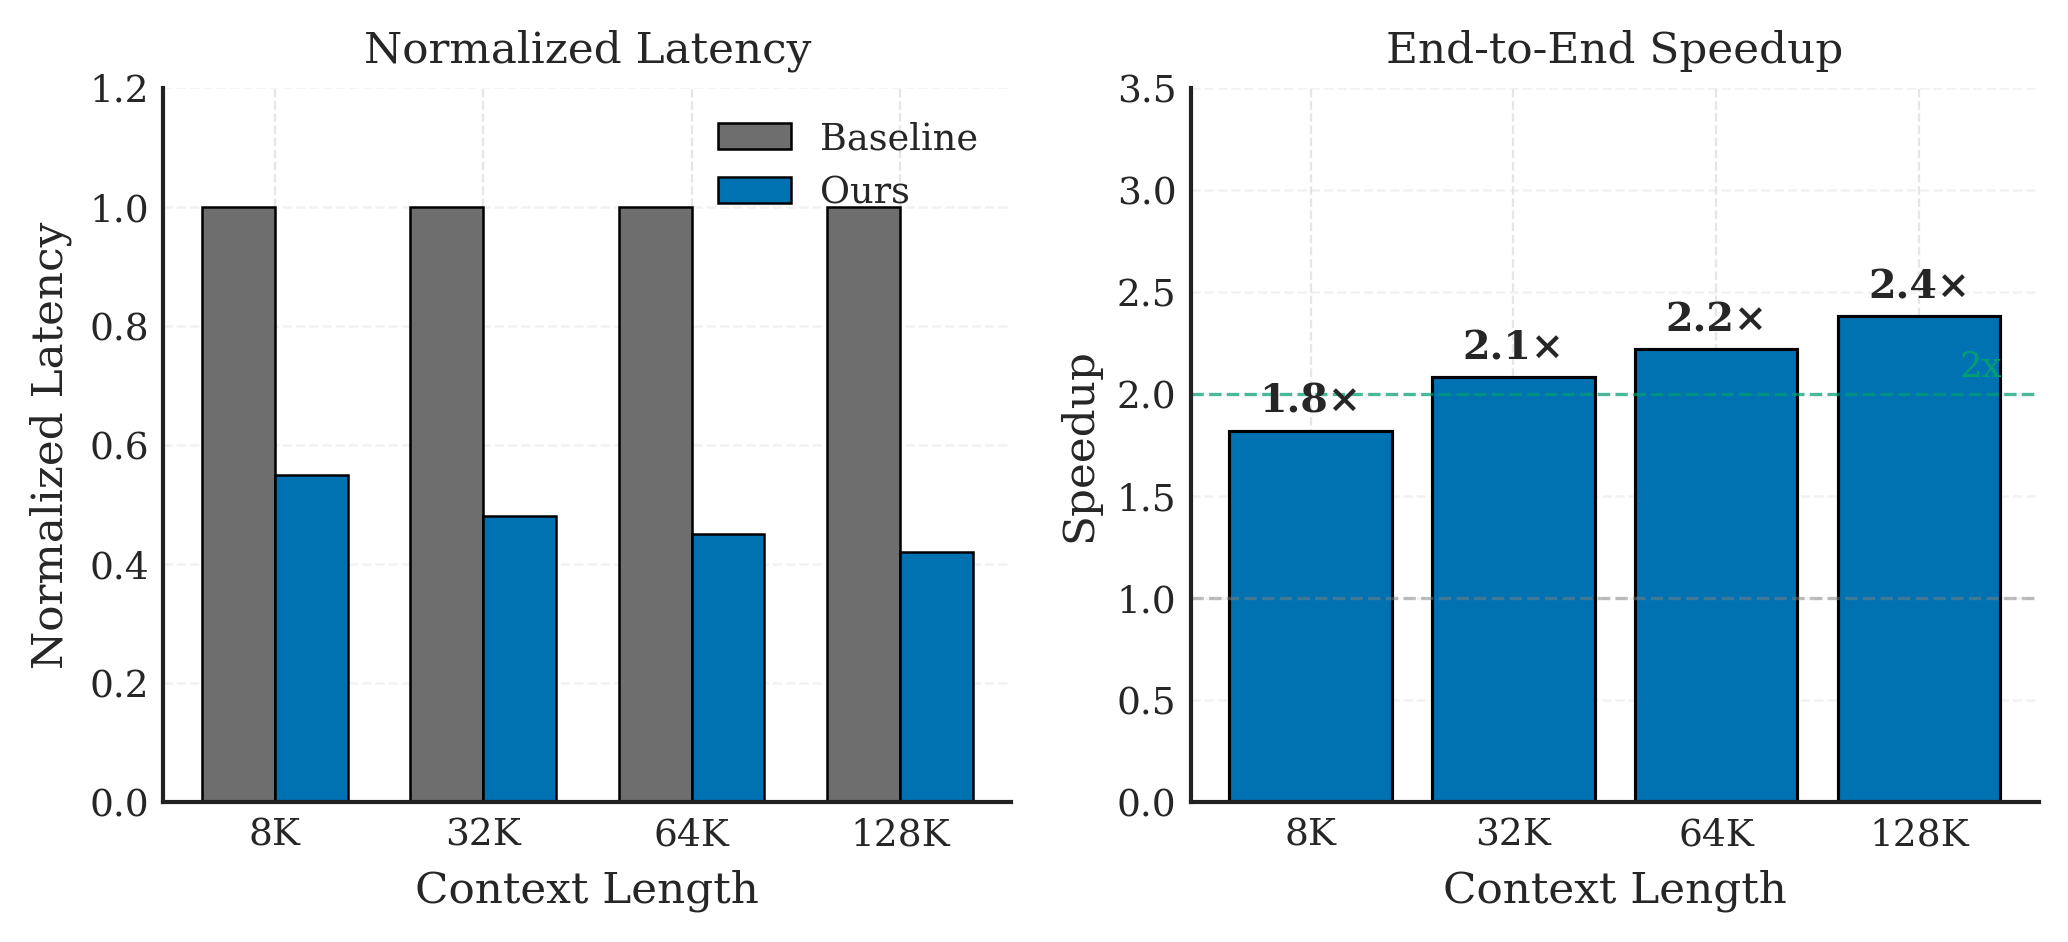
\includegraphics[width=\textwidth]{../paper_assets/figures/fig5_performance_speedup.png}
\caption[Single-node decode speedup]{End-to-end decode speedup of LKC-CXL-PIM relative to the host-aggregated baseline across context lengths.}
\label{fig:performance_speedup}
\end{figure}

Figure~\ref{fig:performance_speedup} reports end-to-end decode speedup. The trend is more important than the absolute value: as context length grows, a larger fraction of the baseline runtime is spent moving KV-cache data rather than computing on it. The measured speedup rises from $1.8\times$ at 8K to $2.4\times$ at 128K, which matches the expectation from the trace profile in Chapter~\ref{ch:motivation}.

\begin{figure}[htbp]
\centering
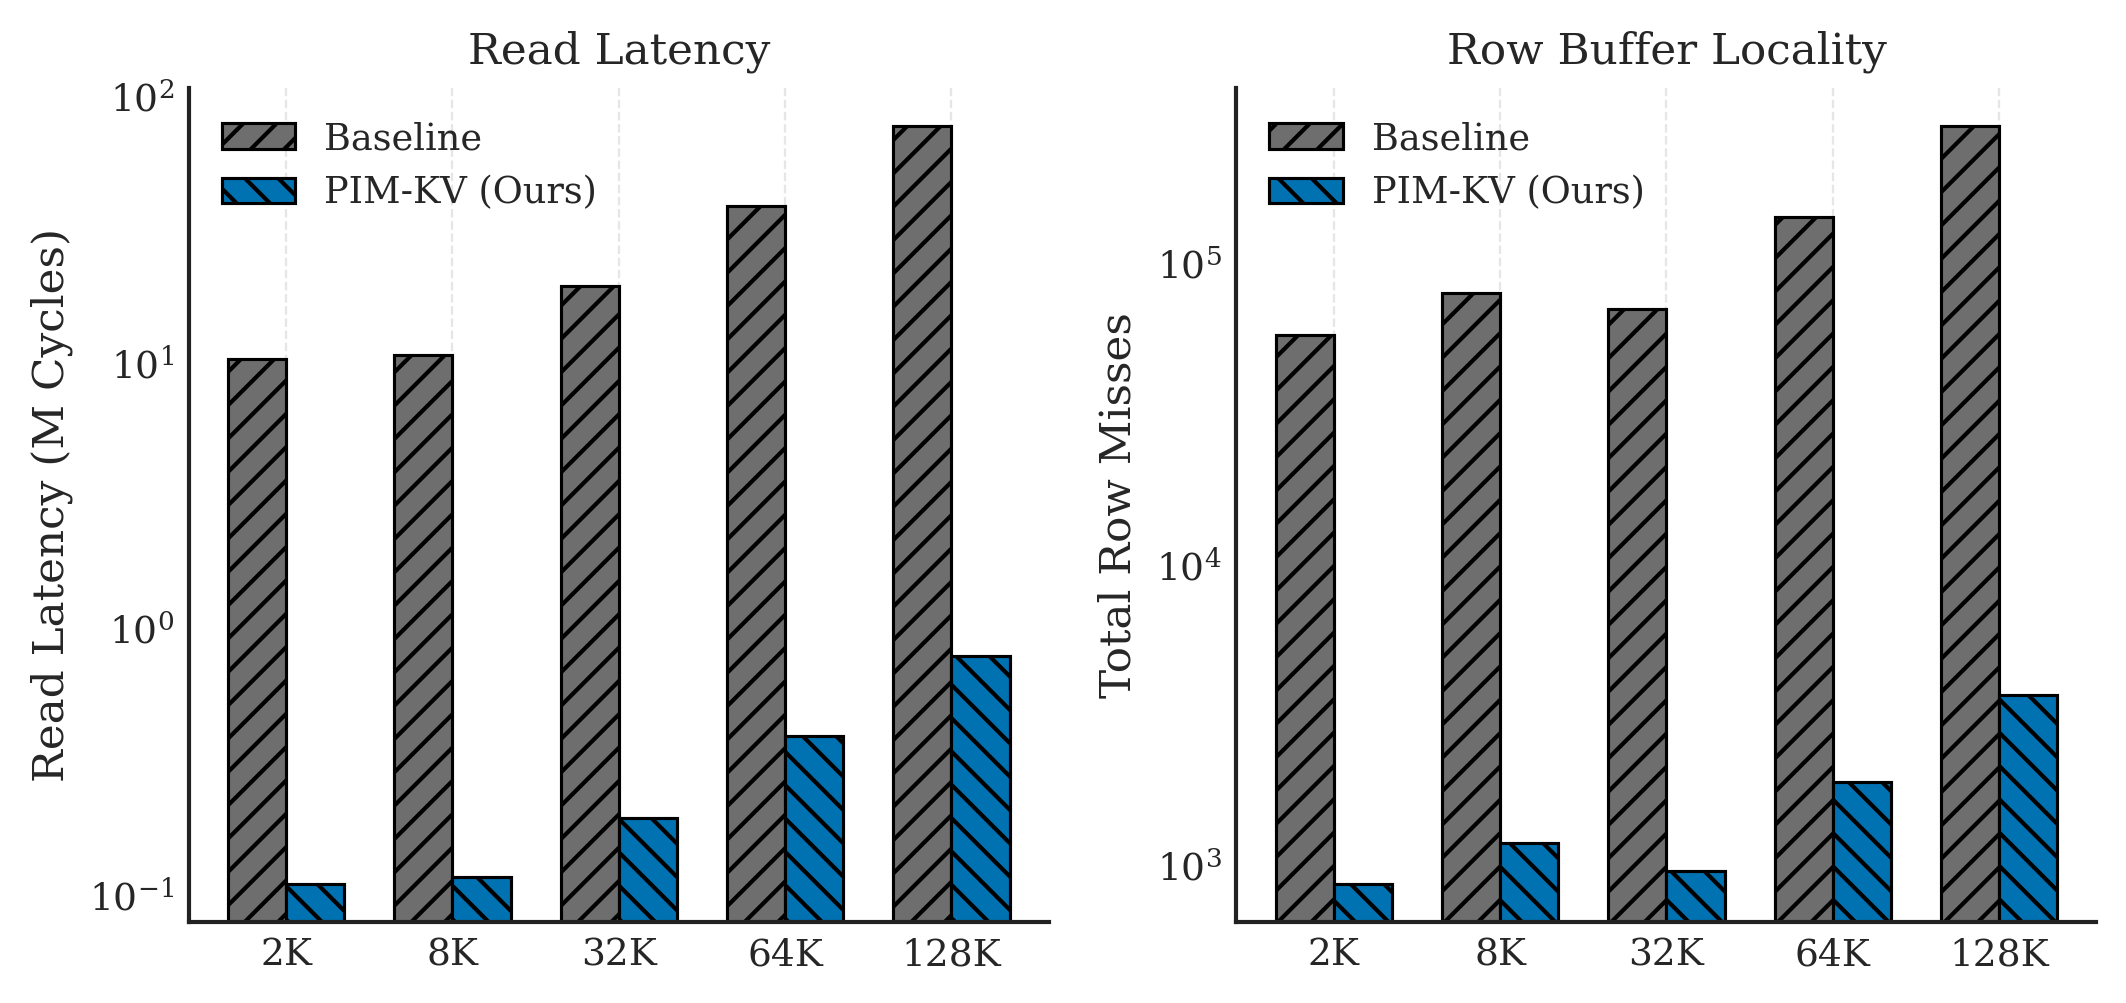
\includegraphics[width=0.9\textwidth]{../paper_assets/figures/fig7_ramulator_comparison.png}
\caption[Cycle-accurate latency comparison]{Cycle-accurate comparison of latency components and row-buffer locality for the baseline and LKC-CXL-PIM.}
\label{fig:ramulator}
\end{figure}

Figure~\ref{fig:ramulator} shows the source of that speedup. At 8K context length, read latency drops from 10.77\,M cycles to 0.12\,M cycles. At 128K, it drops from 77.90\,M cycles to 0.80\,M cycles. The same reorganization also improves row-buffer locality: row misses fall from 80,483 to 1,195 at 8K and from 288,535 to 3,700 at 128K. These reductions are consistent with the intended design goal of keeping KV-cache accesses local to the memory device. They also explain why the result improves with context length: the baseline repeats a larger remote traversal, while LKC-CXL-PIM keeps most of that traversal inside the endpoint.

The difference between the nearly two-order-of-magnitude memory-counter reduction and the more modest end-to-end speedup is expected. Decode still contains non-KV work, host scheduling overhead, and residual synchronization cost. LKC-CXL-PIM therefore does not make generation free; it removes the term that grows most aggressively with context length. This distinction is important because it prevents the memory results from being mistaken for a full application-level speedup.

\section{Area and Energy Efficiency}

\begin{figure}[htbp]
    \centering
    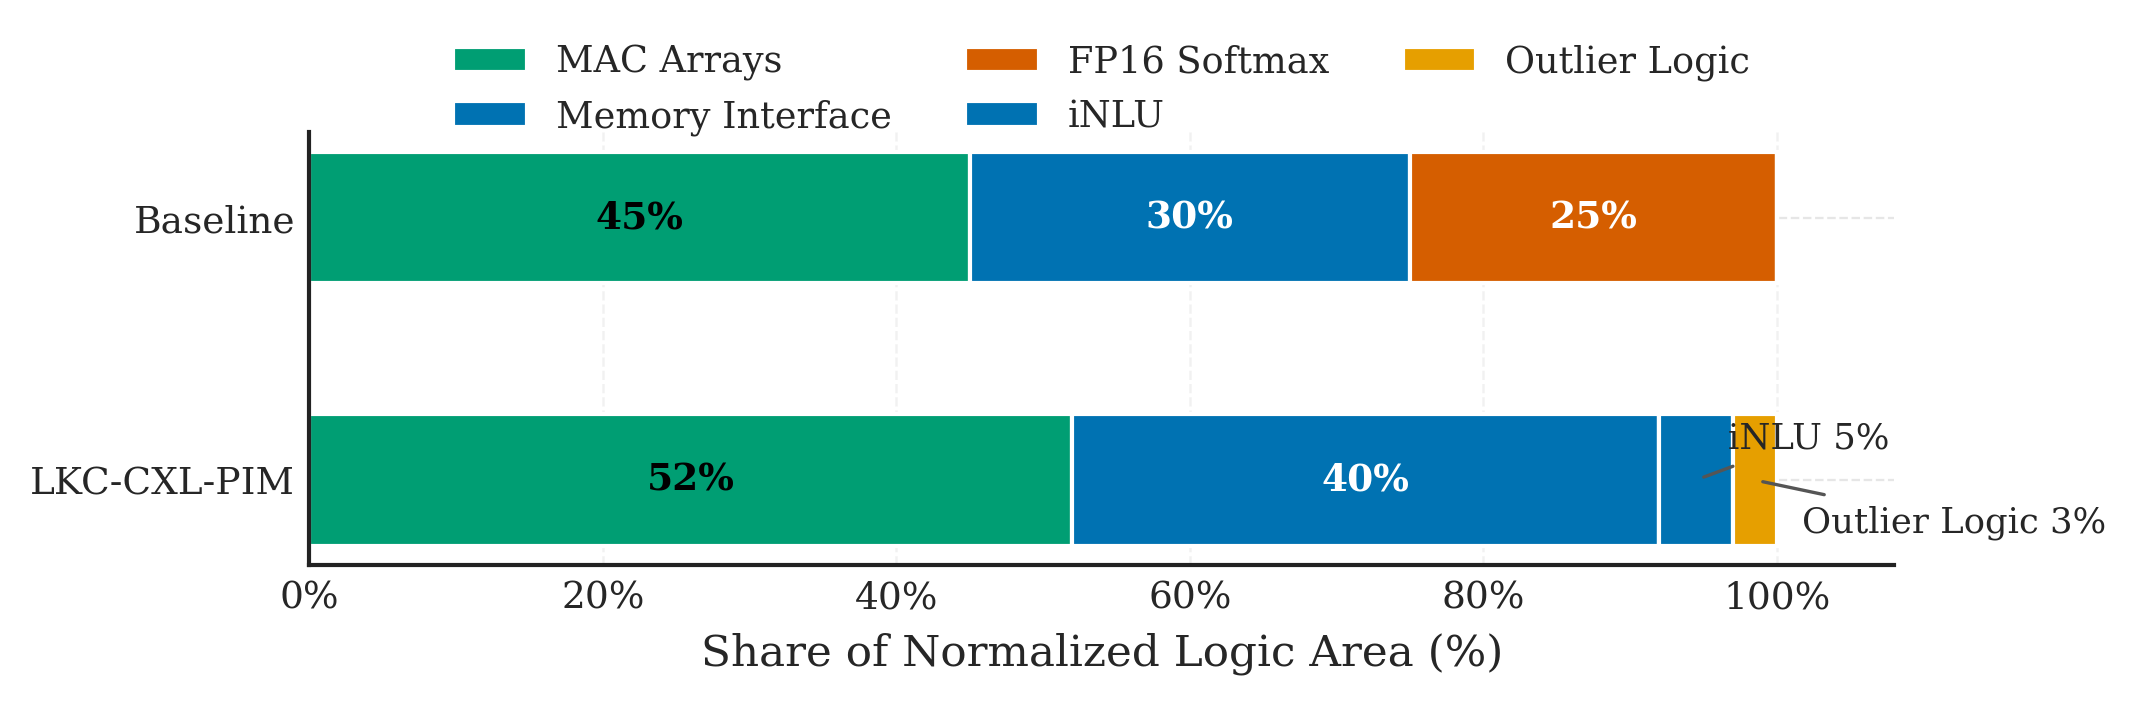
\includegraphics[width=0.92\textwidth]{../paper_assets/figures/fig6_area_breakdown.png}
    \caption[Overall area breakdown]{Overall logic-area breakdown for the baseline softmax path and the LKC-CXL-PIM datapath.}
    \label{fig:area}
\end{figure}

Figure~\ref{fig:area} reports the area breakdown at the logic-die level. In the baseline organization, the FP16 softmax block occupies approximately 25\% of the logic budget. In LKC-CXL-PIM, that block is replaced by the iNLU and outlier-handling path, whose combined footprint is approximately 8\%. The net result is a 17\% overall logic-area reduction even after adding the overflow path.

\begin{figure}[htbp]
    \centering
    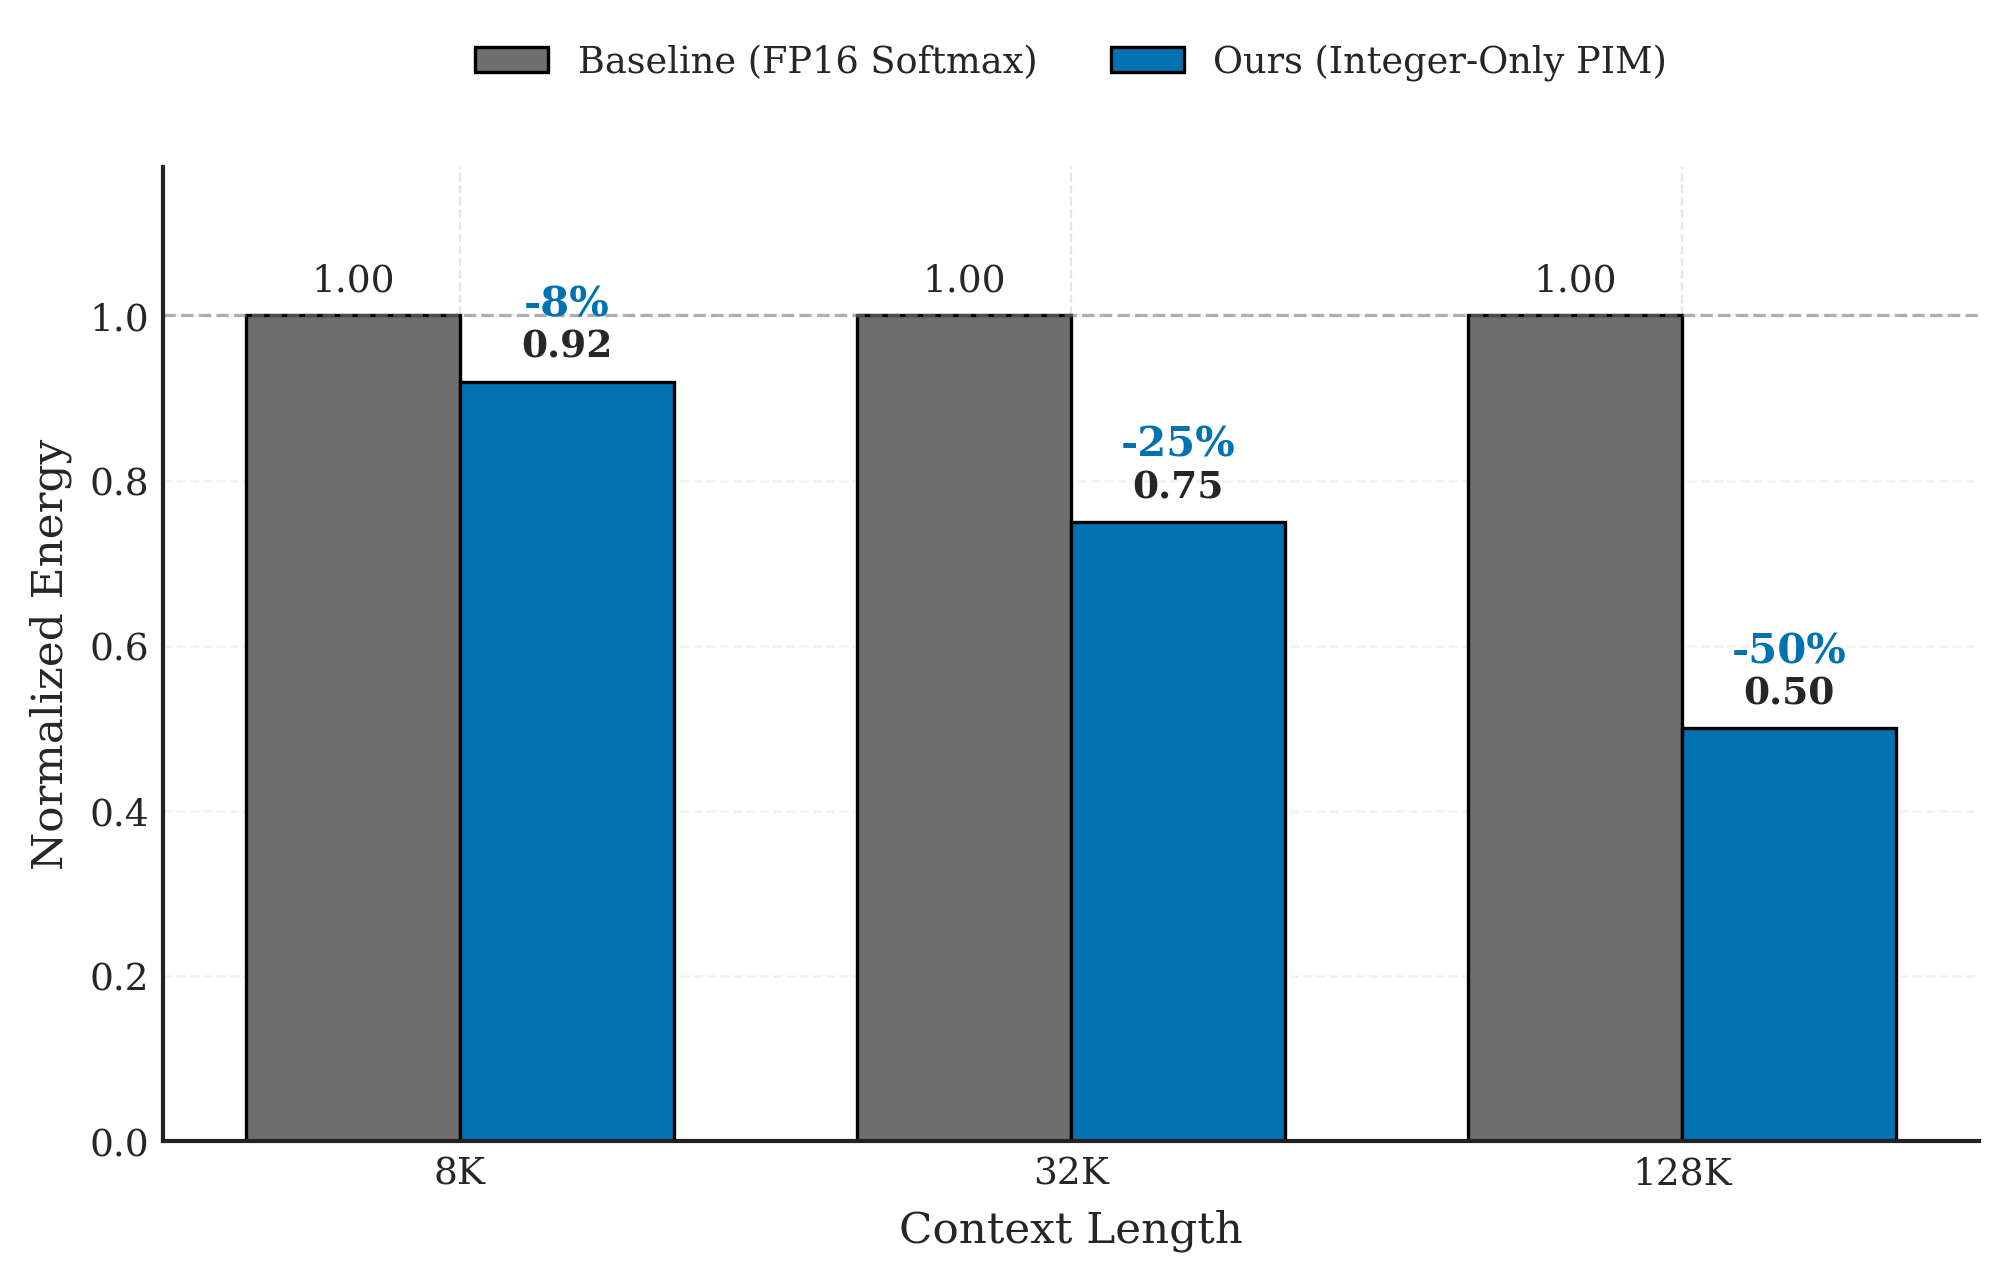
\includegraphics[width=0.78\textwidth]{../paper_assets/figures/fig2_energy_comparison.png}
    \caption[Normalized energy by context length]{Normalized energy consumption across representative context lengths.}
    \label{fig:energy}
\end{figure}

Figure~\ref{fig:energy} shows the corresponding energy trend. The measured normalized savings are 8.3\% at 8K, 24.9\% at 32K, and approximately 50.0\% at 128K. The savings increase with context length because the avoided off-package traffic grows with the size of the historical KV cache.

Area and energy move in the same direction for different reasons. Area improves because the floating-point nonlinear path is replaced by a smaller fixed-point approximation and a small overflow buffer. Energy improves mainly because the design avoids repeated link traversal of the historical KV state. This distinction matters: the endpoint logic is not free, but in the evaluated setting it is small enough that reduced movement dominates the trade-off.

\section{iNLU Mathematical Fidelity}

\begin{figure}[htbp]
    \centering
    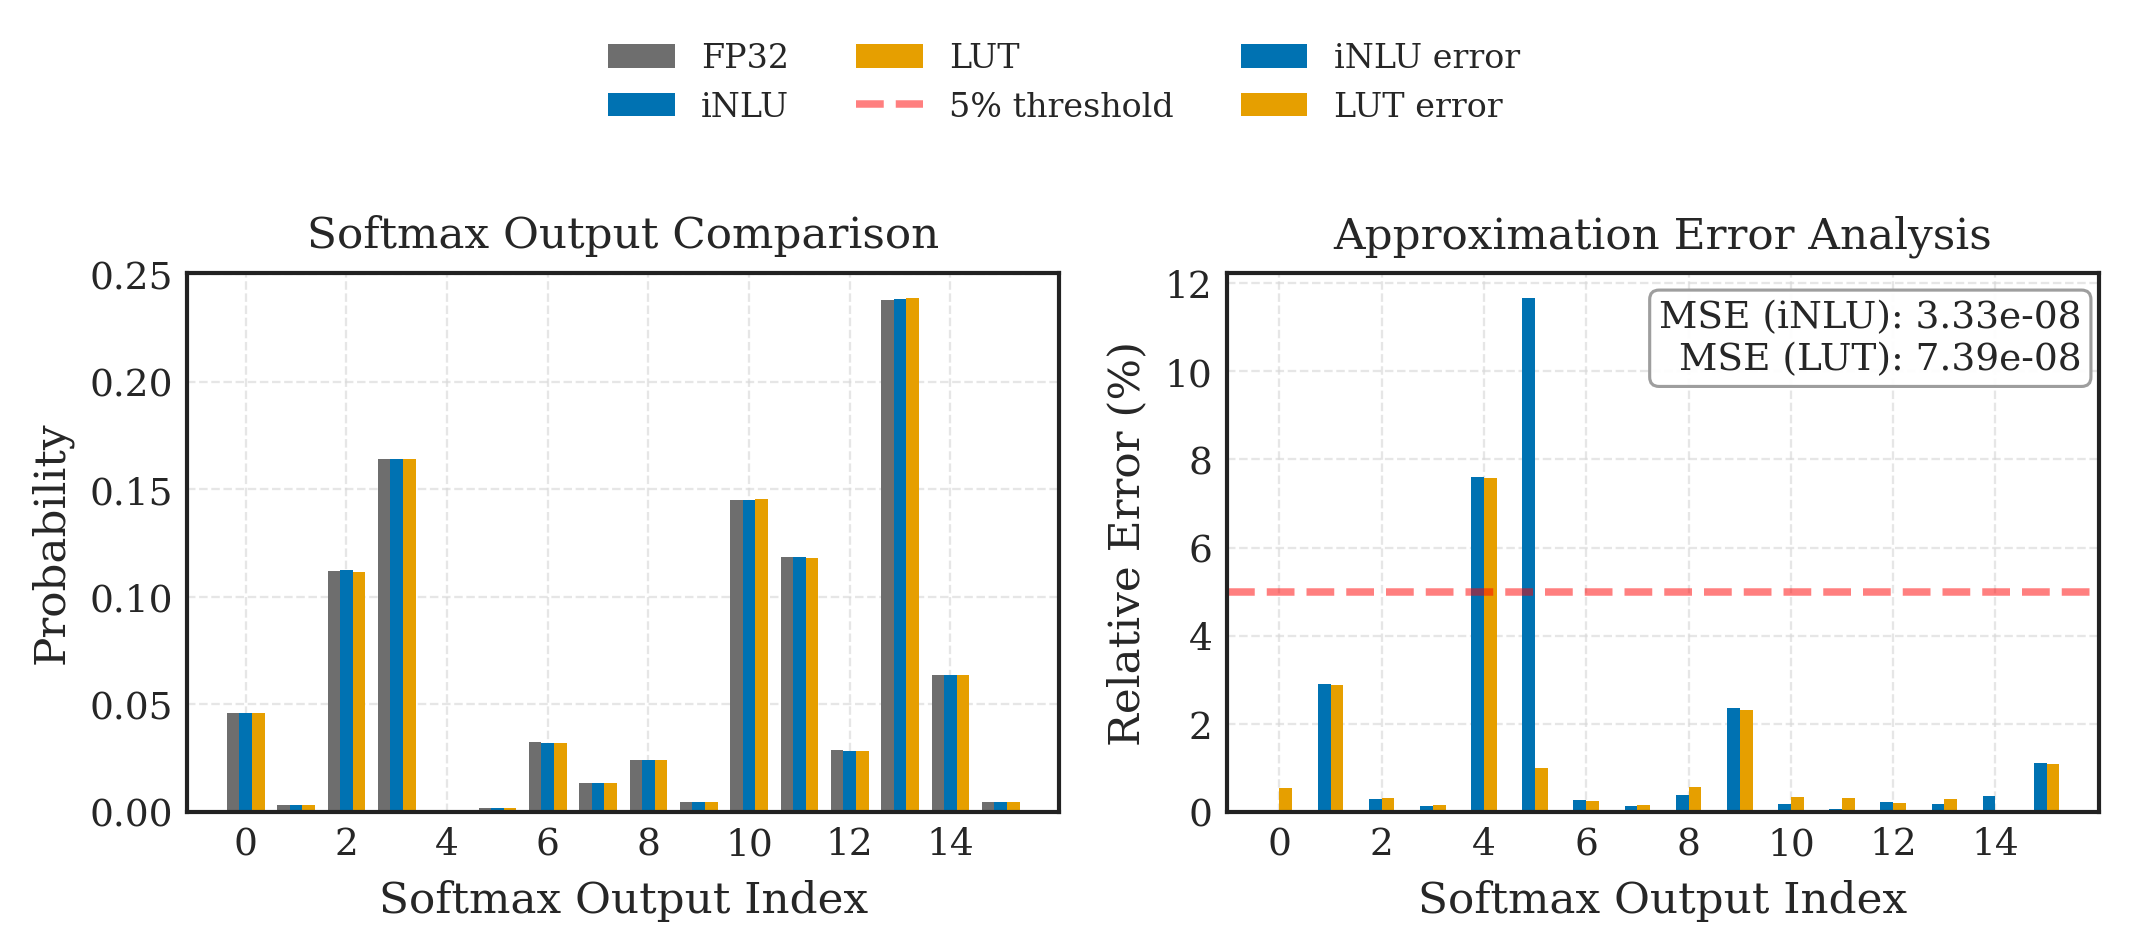
\includegraphics[width=0.9\textwidth]{../paper_assets/figures/fig4_inlu_accuracy.png}
    \caption[iNLU softmax-approximation fidelity]{Softmax output comparison and approximation error for the iNLU polynomial path versus a lookup-table approximation.}
    \label{fig:inlu_acc}
\end{figure}

\begin{figure}[htbp]
    \centering
    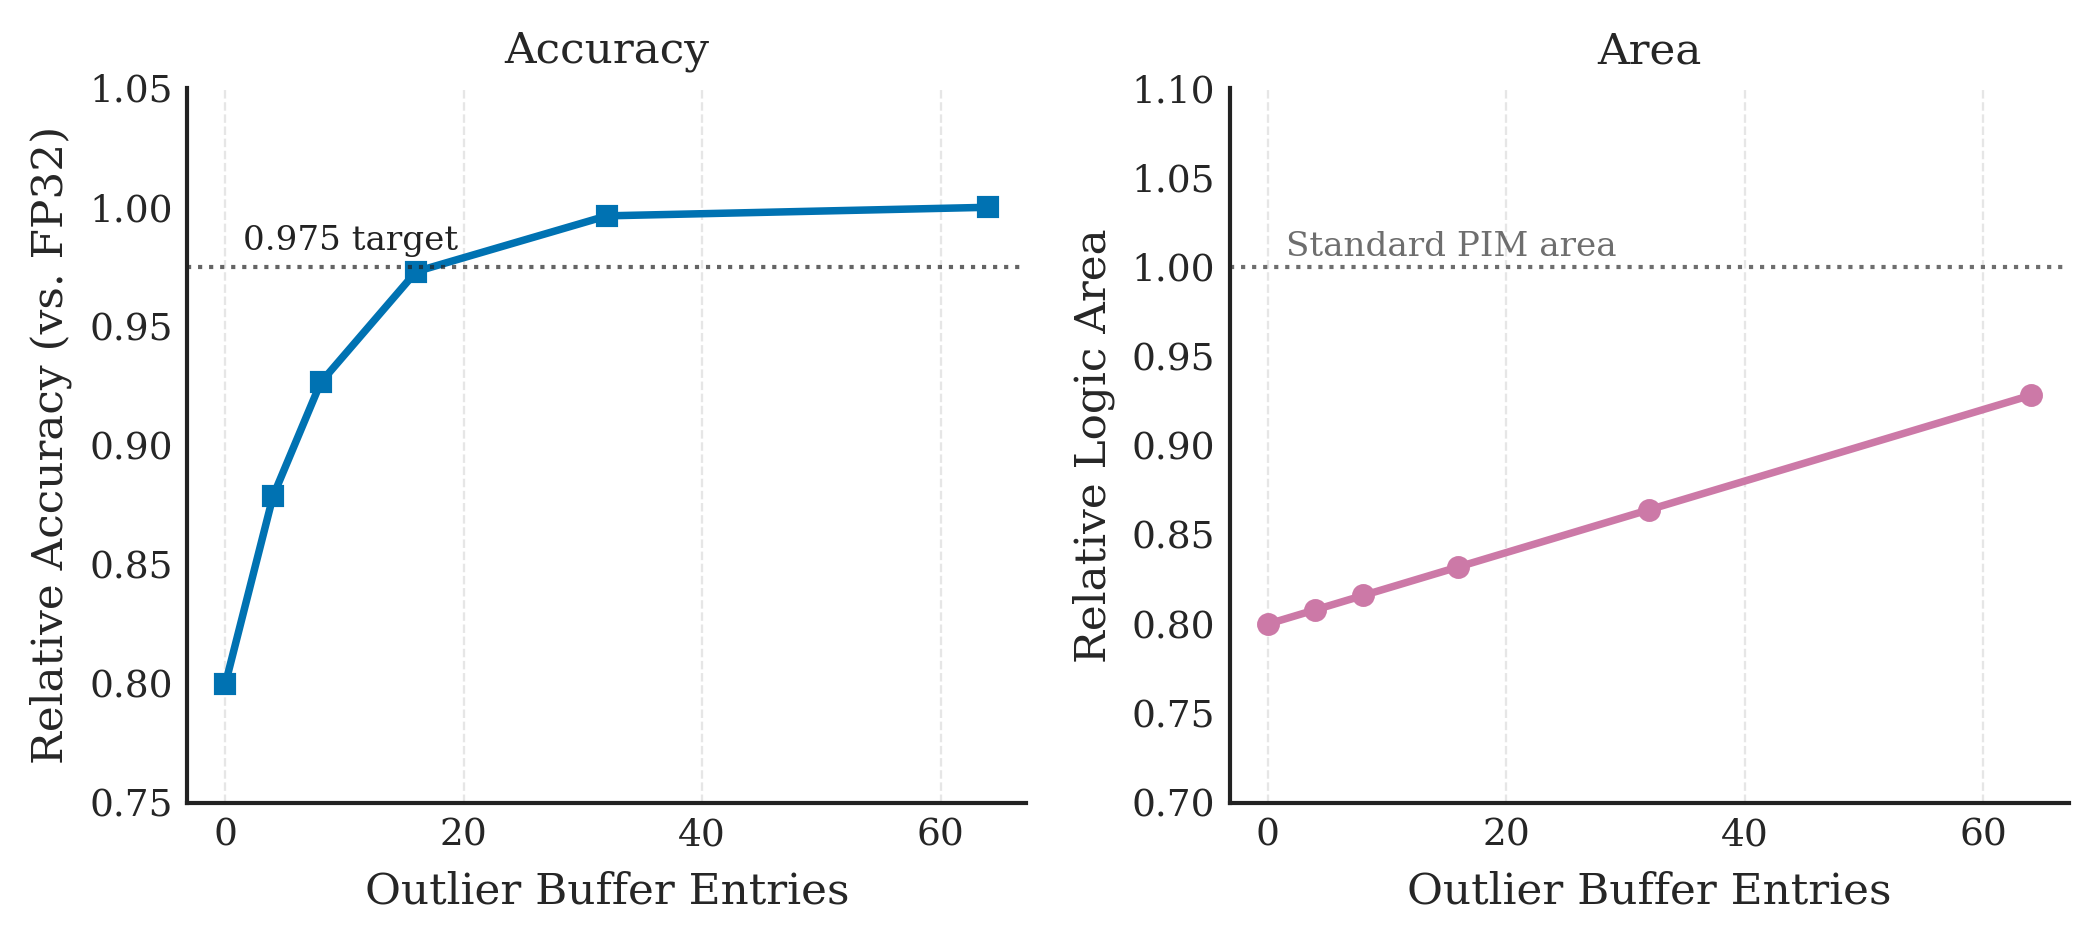
\includegraphics[width=0.9\textwidth]{../paper_assets/figures/fig10_sensitivity_outliers.png}
    \caption[Outlier-buffer sensitivity]{Sensitivity of relative accuracy and relative area to the size of the outlier buffer.}
    \label{fig:sens_outliers}
\end{figure}

\begin{figure}[htbp]
    \centering
    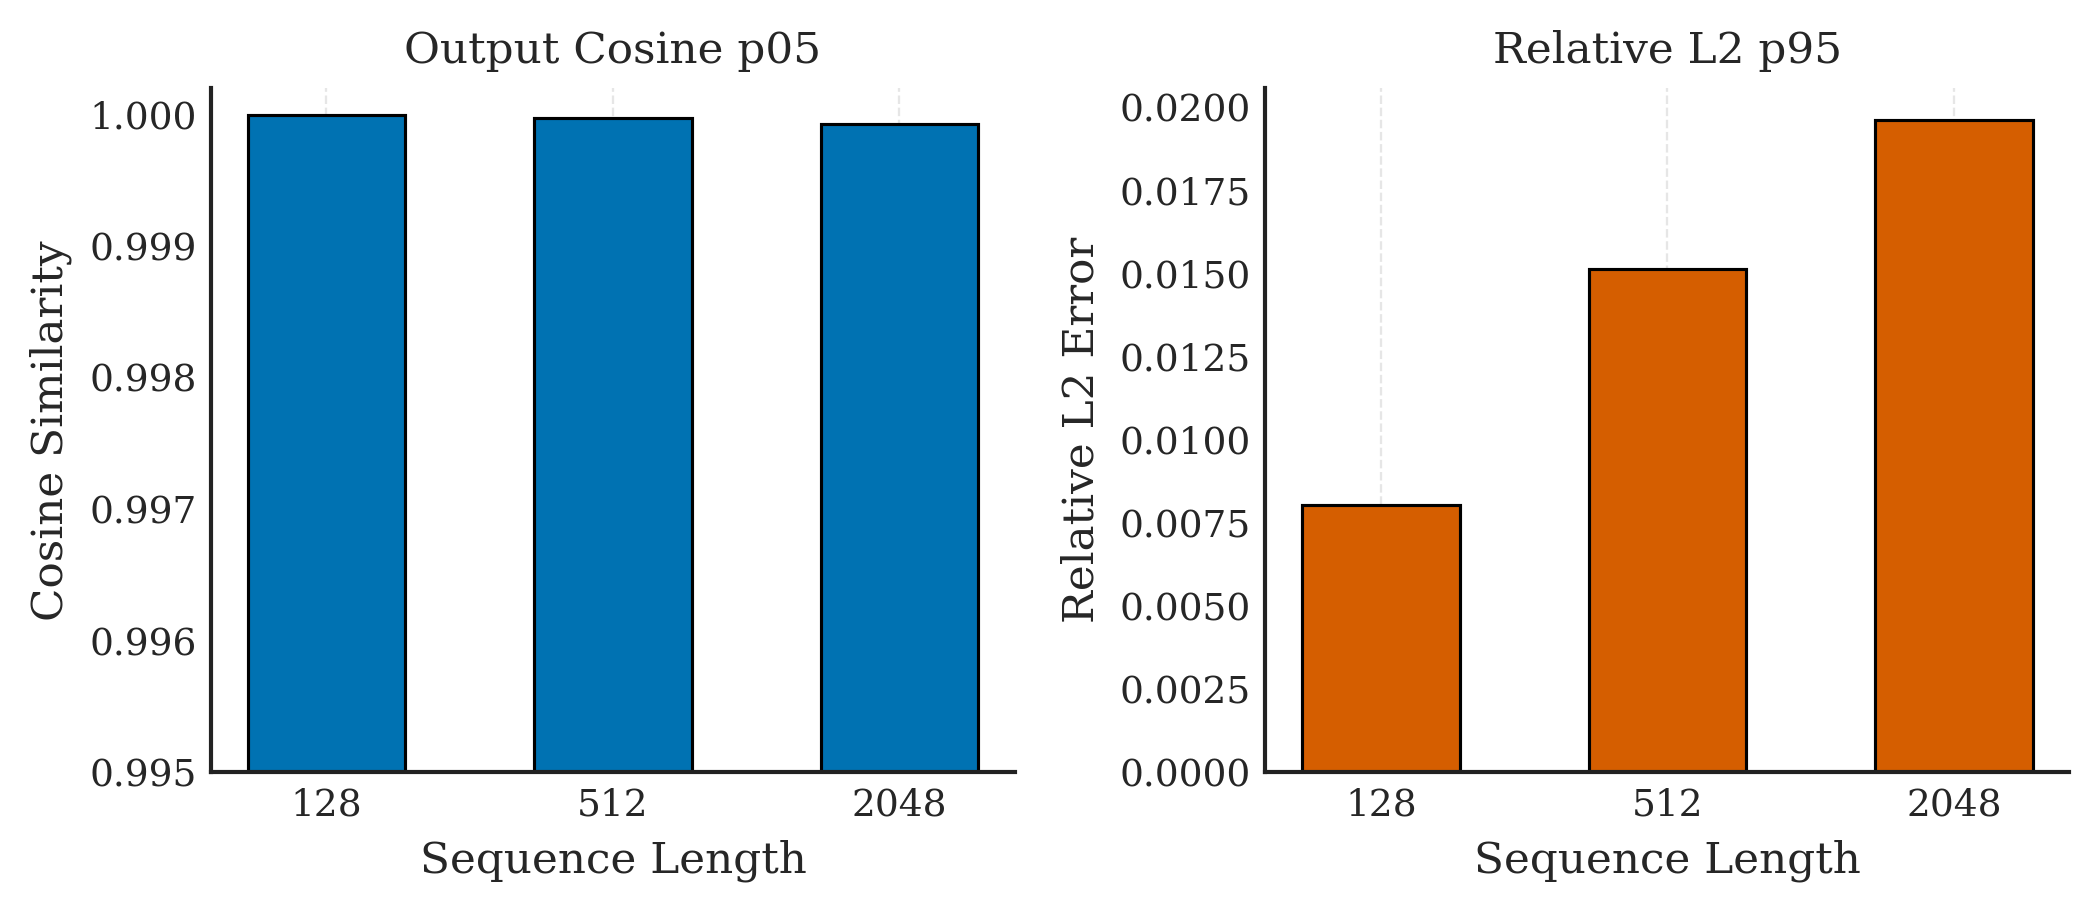
\includegraphics[width=0.78\textwidth]{../paper_assets/figures/fig11_attention_quality.png}
    \caption[Attention-output quality under fixed-point iNLU]{Attention-output quality of the fixed-point iNLU path across sequence lengths.}
    \label{fig:attention_quality}
\end{figure}

Figure~\ref{fig:inlu_acc} checks whether the integer approximation is accurate enough for attention normalization. The plotted iNLU path uses the fixed-point golden model with Q10 logits, the integer polynomial exponential, and Q24 integer normalization. It tracks the FP32 reference closely and has lower mean-squared error than the 64-entry lookup-table alternative in the same figure, about $3.33\times10^{-8}$ versus $7.39\times10^{-8}$. This matters because it addresses the most direct objection to iNLU: the area reduction is not coming from an obviously coarse exponential approximation.

Figure~\ref{fig:attention_quality} moves the check from softmax error to attention behavior. I ran the same fixed-point path in a lightweight single-head Q/K/V attention benchmark over 128, 512, and 2048-token sequences. Across 128 trials per sequence length, the worst 5th-percentile output-vector cosine similarity stays above 0.99992, and the worst 95th-percentile relative $\ell_2$ output error is 1.96\%. This is not a substitute for full language-model perplexity evaluation, but it shows that the integer normalization error remains small at the attention-output level.

Figure~\ref{fig:sens_outliers} isolates the overflow path. A pure INT8 path starts near 0.80 relative accuracy. Adding a 16-entry buffer raises the result to roughly 0.97 while staying near the relative area of the standard PIM baseline. Larger 32-entry and 64-entry buffers approach full relative accuracy, but the gain beyond 16 entries is smaller than the area cost. I therefore use the 16-entry buffer as the practical operating point in the evaluated design.

\section{Multi-Node Scaling and Throughput}

\begin{figure}[htbp]
    \centering
    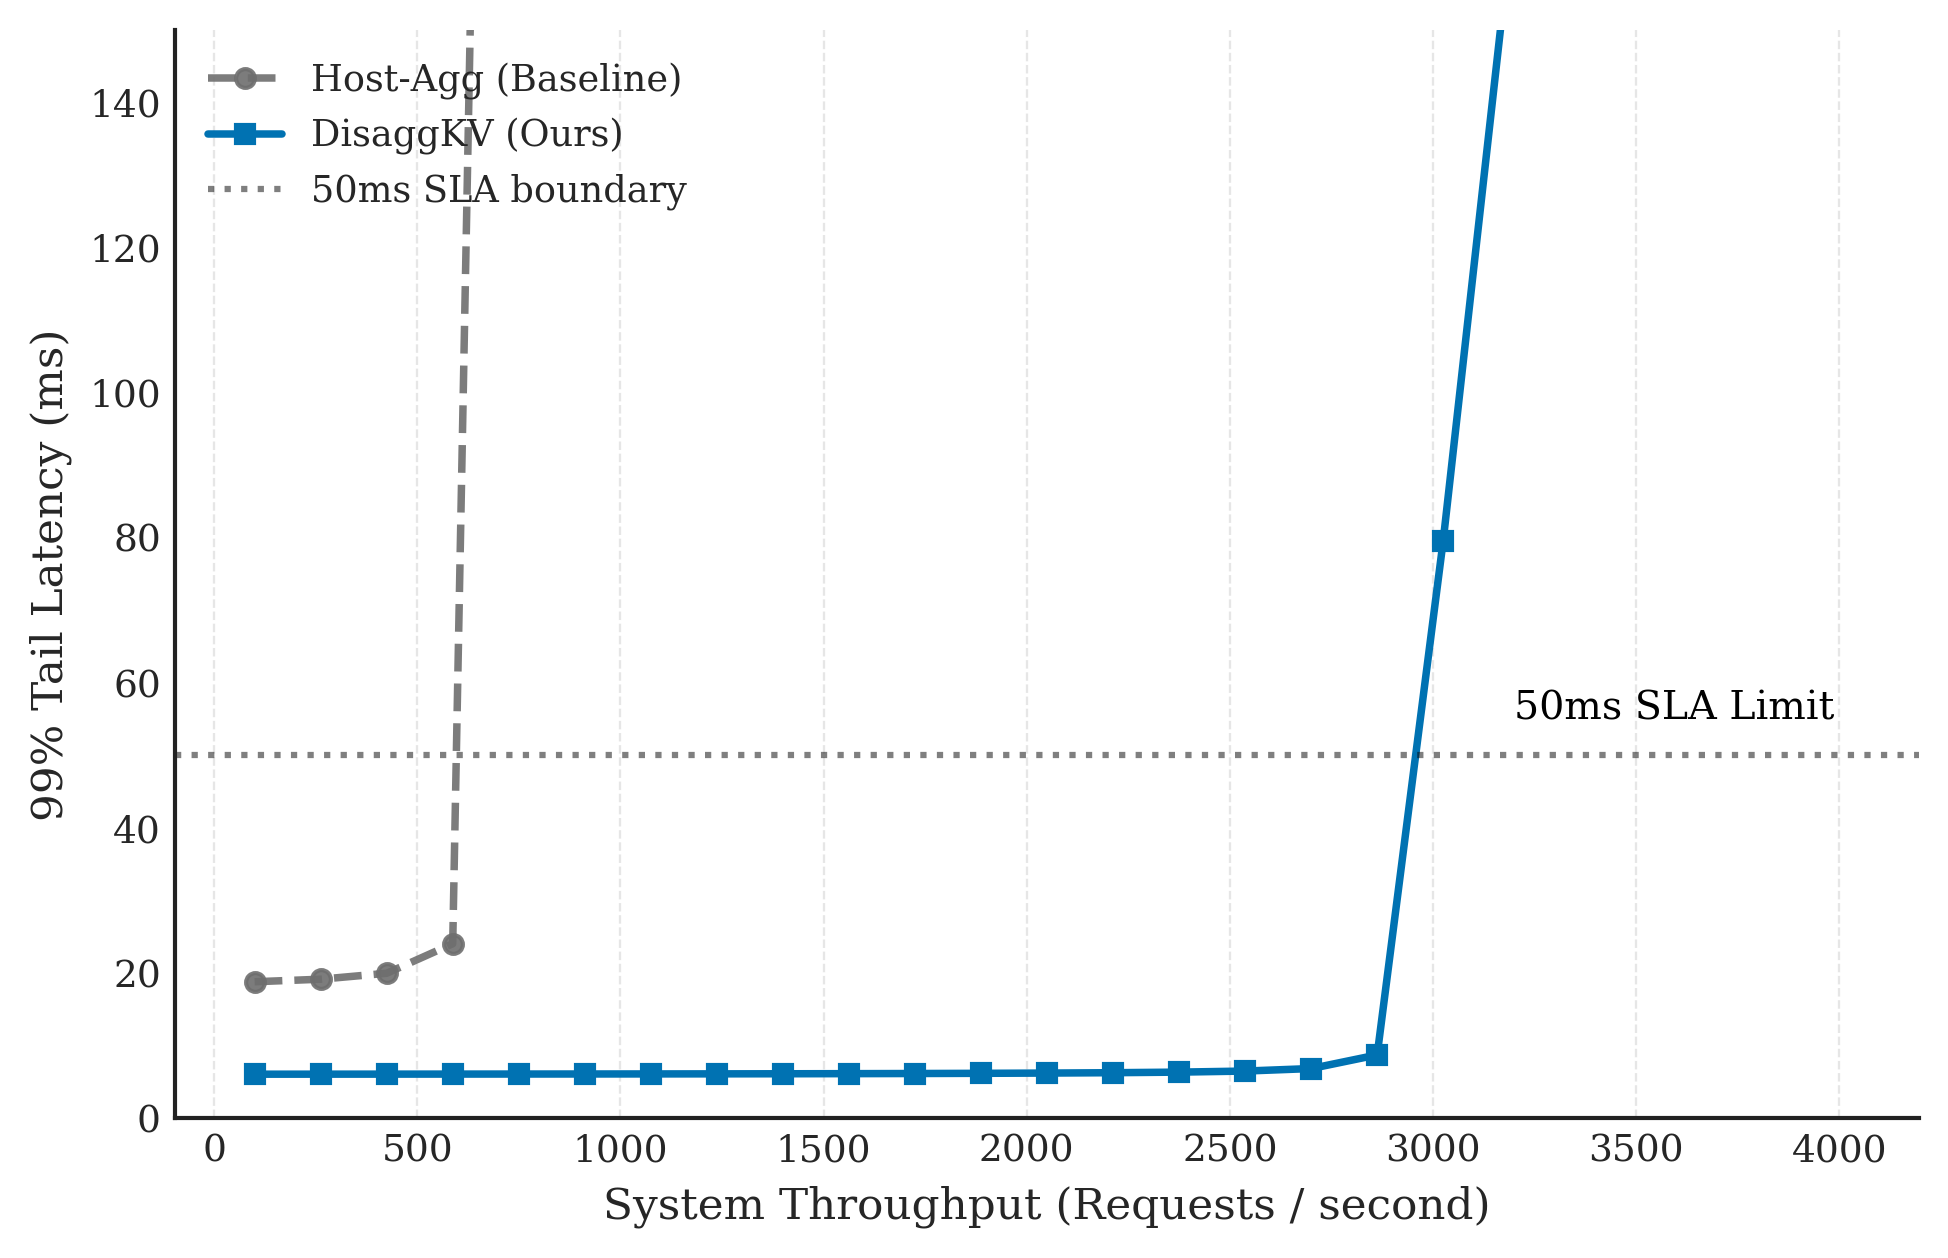
\includegraphics[width=0.82\textwidth]{../paper_assets/figures/fig1_throughput_latency.png}
    \caption[Tail latency versus throughput]{Tail-latency versus throughput for the host-aggregated baseline and DisaggKV.}
    \label{fig:throughput}
\end{figure}

Figure~\ref{fig:throughput} compares modeled throughput and 99th-percentile tail latency using the calibrated queueing model from Chapter~\ref{ch:methodology}. The host-aggregated baseline crosses the 50\,ms SLA boundary slightly above 600 requests/s. DisaggKV remains below 10\,ms through 2.7K requests/s and stays below the 50\,ms target until just under 3.0K requests/s. I compare the designs at the SLA crossing point rather than at the highest plotted point, because that is closer to the operating region a serving system would choose. On that basis, DisaggKV gives roughly a $4.5\times$ throughput improvement over the baseline.

\begin{figure}[htbp]
    \centering
    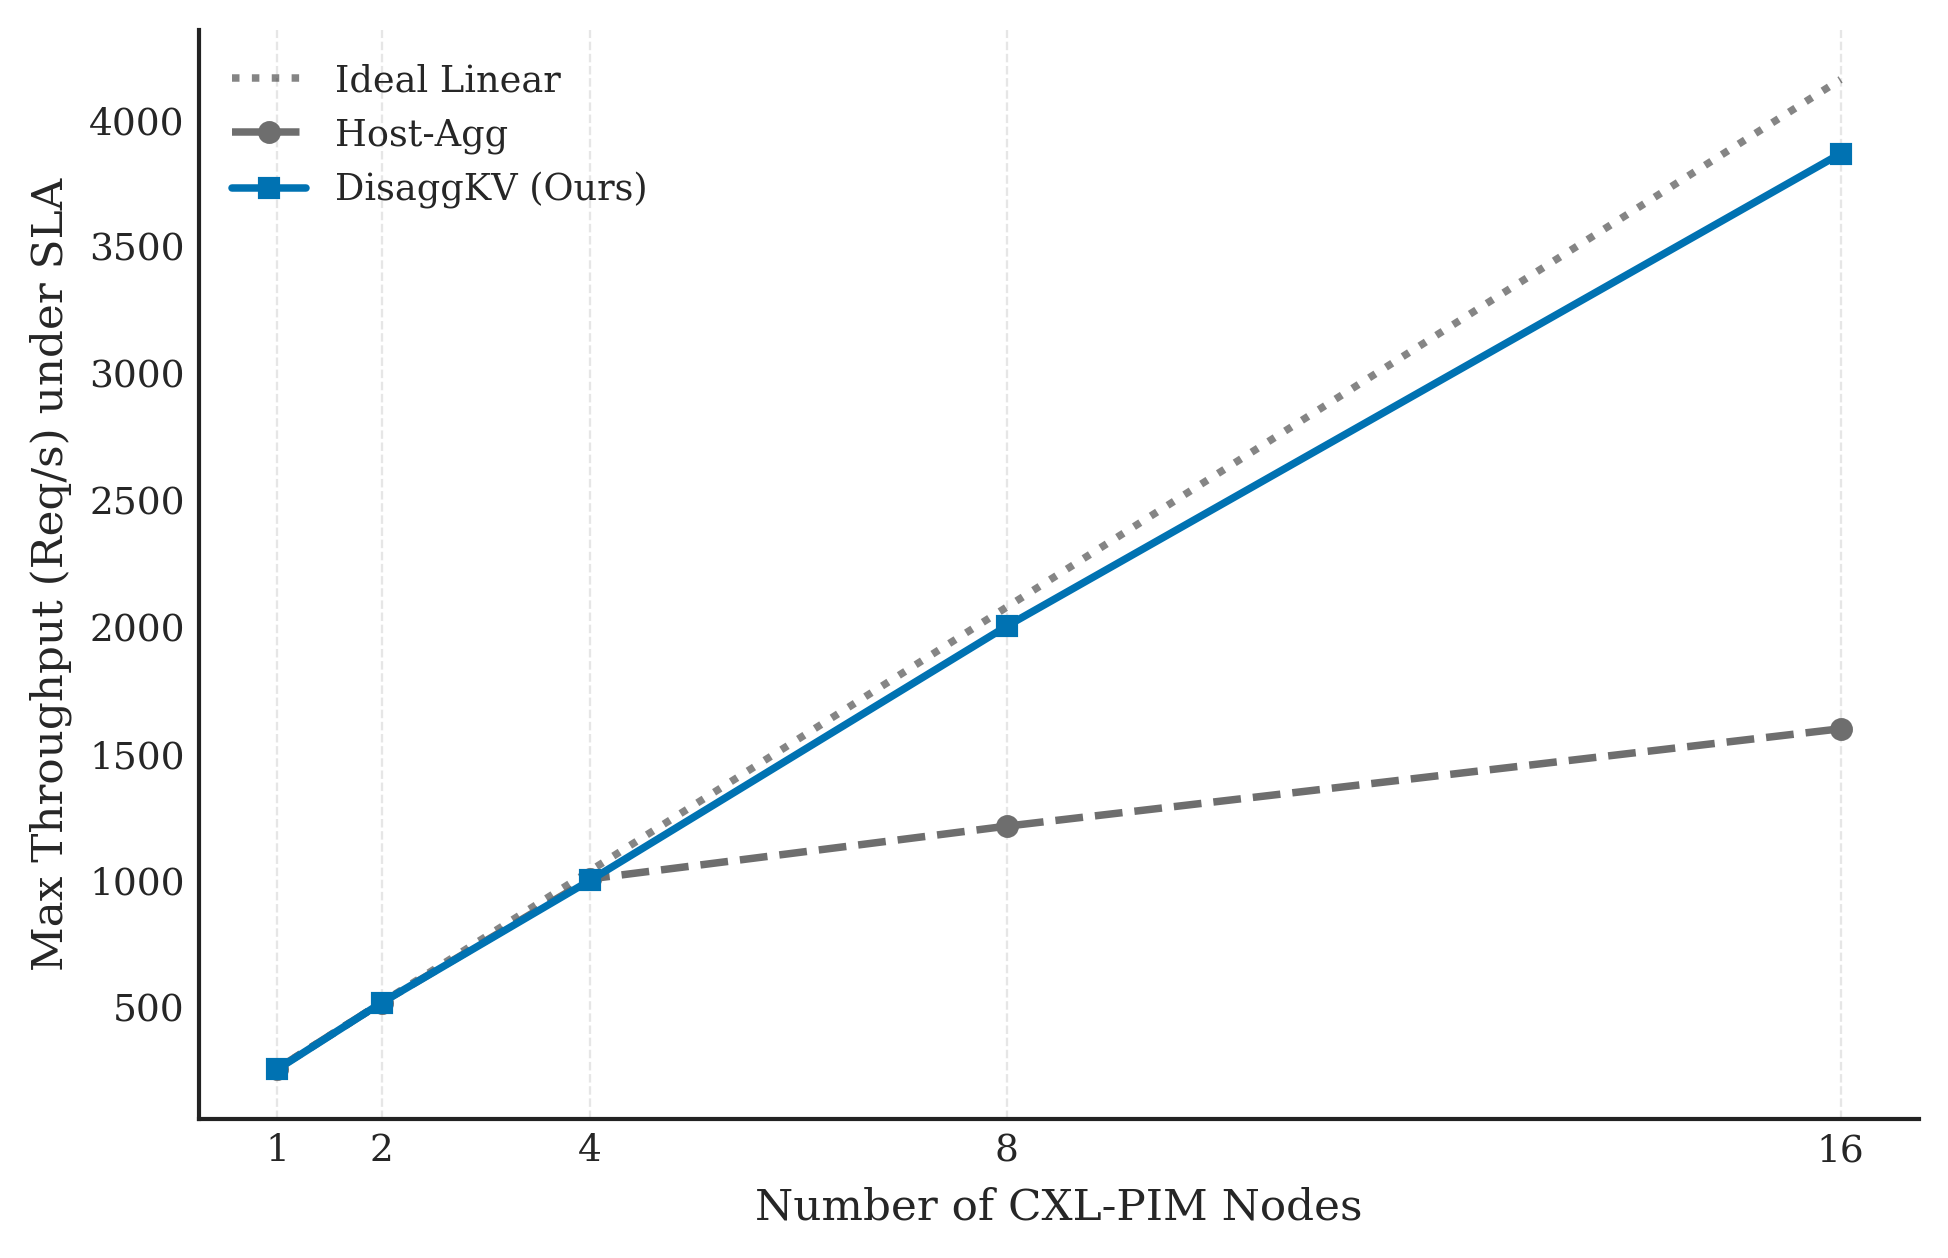
\includegraphics[width=0.82\textwidth]{../paper_assets/figures/fig2_scalability.png}
    \caption[Distributed scalability]{Endpoint-count sweep for DisaggKV in the checked CXL fabric model.}
    \label{fig:scalability}
\end{figure}

Figure~\ref{fig:scalability} plots the endpoint-count sweep. One endpoint serves 257.4 requests/s; eight endpoints reach 2004.9 requests/s, or $7.79\times$ higher throughput. With sixteen endpoints the run reaches 3867.7 requests/s. The useful detail is the change after eight endpoints: capacity and HBM service keep increasing, but reduction barriers start to pull the curve away from an ideal line.

Synchronization explains the bend after eight endpoints. Each added node participates in the two softmax barriers described in Chapter~\ref{ch:disaggkv_system}. DisaggKV keeps those barriers small by exchanging scalars instead of tensors, but it still has to wait for them. The scaling curve is therefore close to linear through eight nodes and visibly below the ideal line at sixteen.

\section{Traffic Accounting and Local Recovery}

\begin{figure}[htbp]
    \centering
    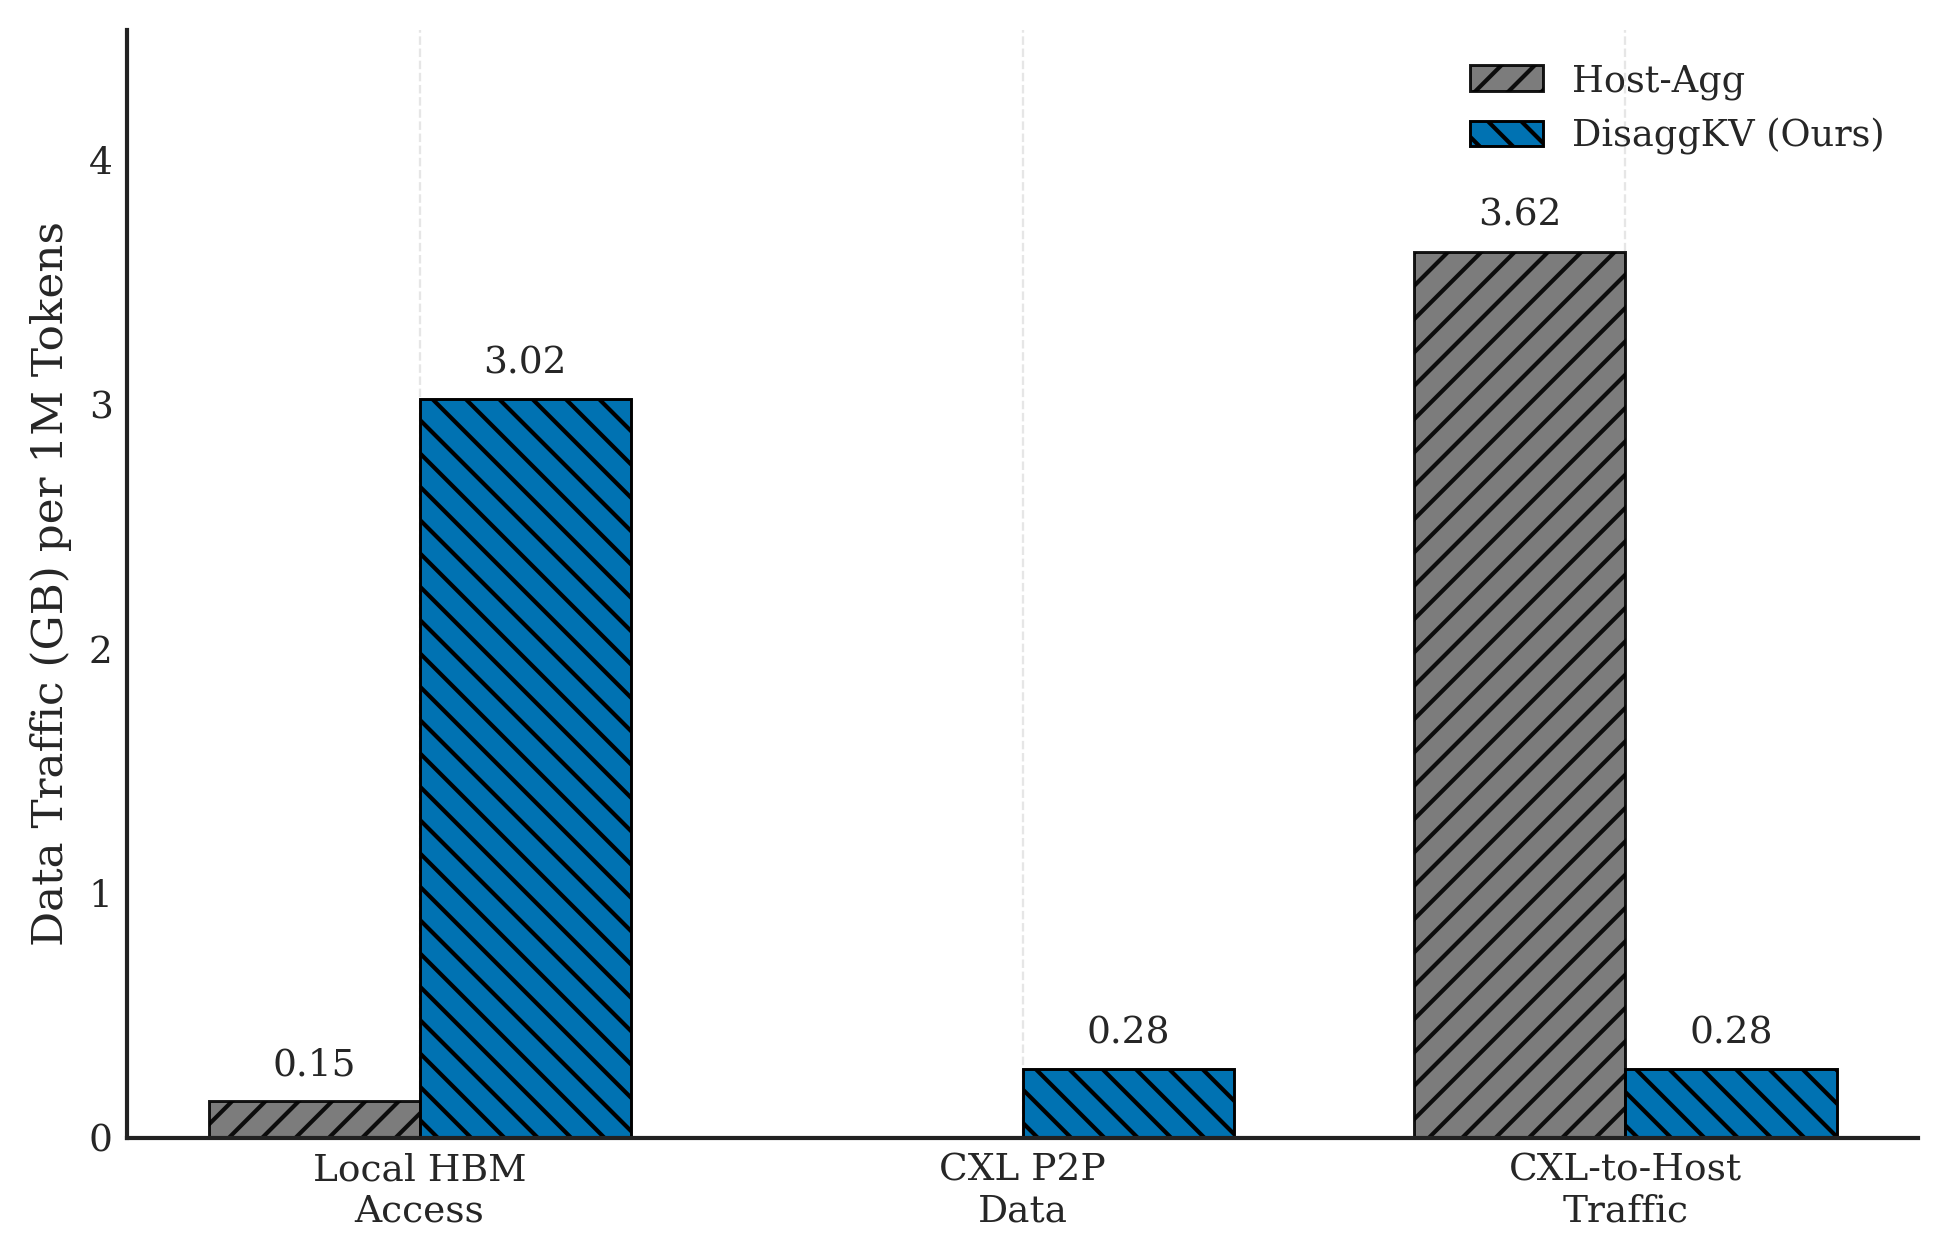
\includegraphics[width=0.82\textwidth]{../paper_assets/figures/fig3_network_breakdown.png}
    \caption[Interconnect traffic breakdown]{Local-HBM, peer-to-peer, and host-facing bytes per 1M decoded tokens in the CXL artifact.}
    \label{fig:network_break}
\end{figure}

The traffic accounting in Figure~\ref{fig:network_break} explains why the latency curve moves. Local HBM access increases because more of the attention work completes on the memory endpoints. Host-facing CXL traffic, however, falls from 3.624\,GB to 0.282\,GB per 1M tokens, a 92.2\% reduction. Even after peer-to-peer reduction traffic is counted, total interconnect traffic remains about 84.4\% below the host-aggregated baseline. These values come from the checked-in CXL fabric artifact and are normalized by the token count of the 50-request trace.

\begin{figure}[htbp]
    \centering
    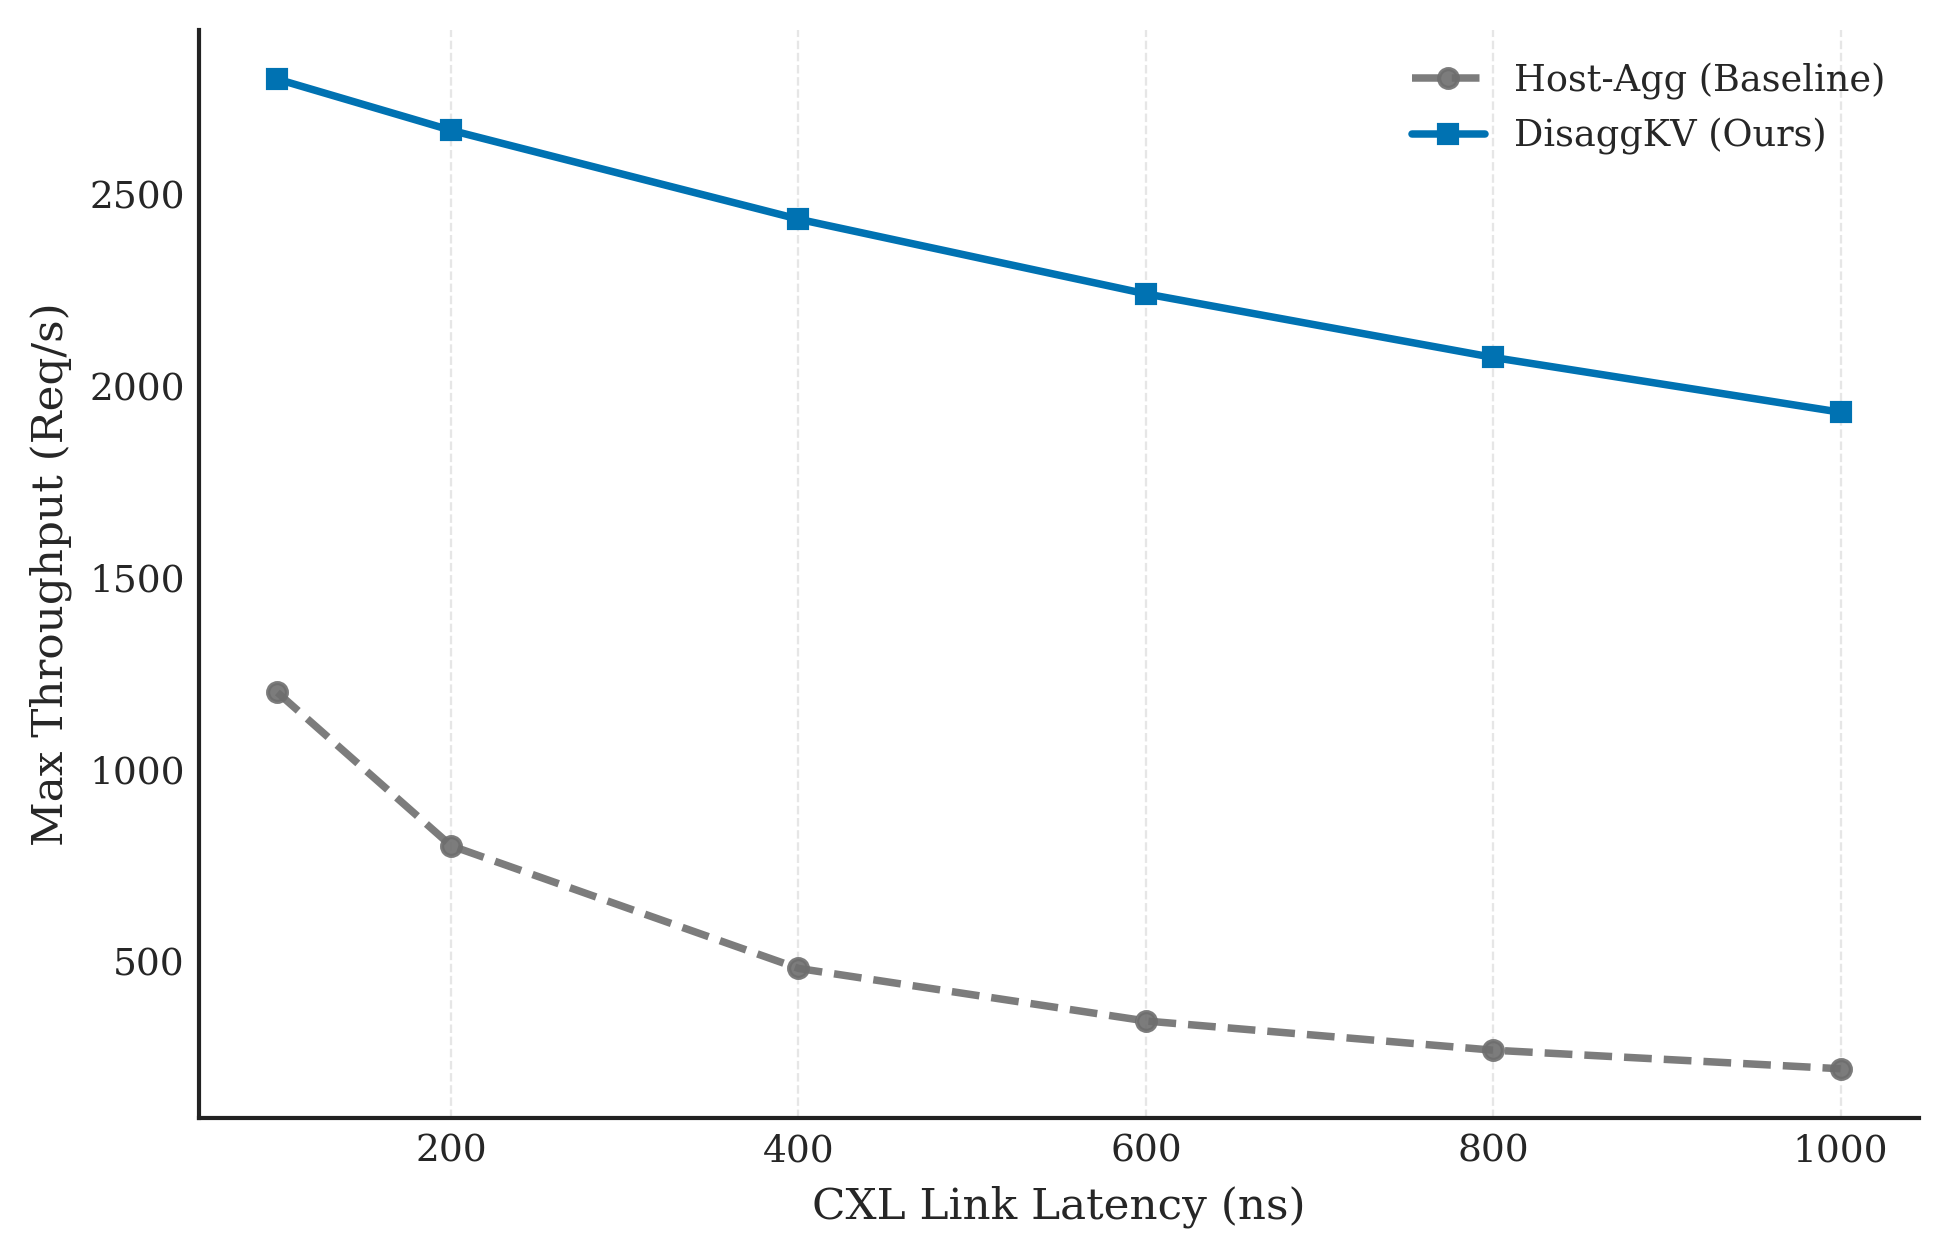
\includegraphics[width=0.82\textwidth]{../paper_assets/figures/fig5_sensitivity_latency.png}
    \caption[Latency-sensitivity study]{Throughput of both designs when modeled CXL-link latency is swept from 100\,ns to 1\,$\mu$s.}
    \label{fig:sens_latency}
\end{figure}

The latency sweep in Figure~\ref{fig:sens_latency} uses the same workload while stretching the CXL-link delay from 100\,ns to 1\,$\mu$s. Under that sweep, the host-aggregated baseline drops from roughly 1200 to 230 requests/s, while DisaggKV drops from roughly 2780 to 1930 requests/s. DisaggKV is not latency-insensitive, since the reduction barriers still cross the fabric. It tolerates the sweep better because its communication pattern is dominated by compact scalar reduction rather than dense tensor fetches.

\begin{figure}[htbp]
\centering
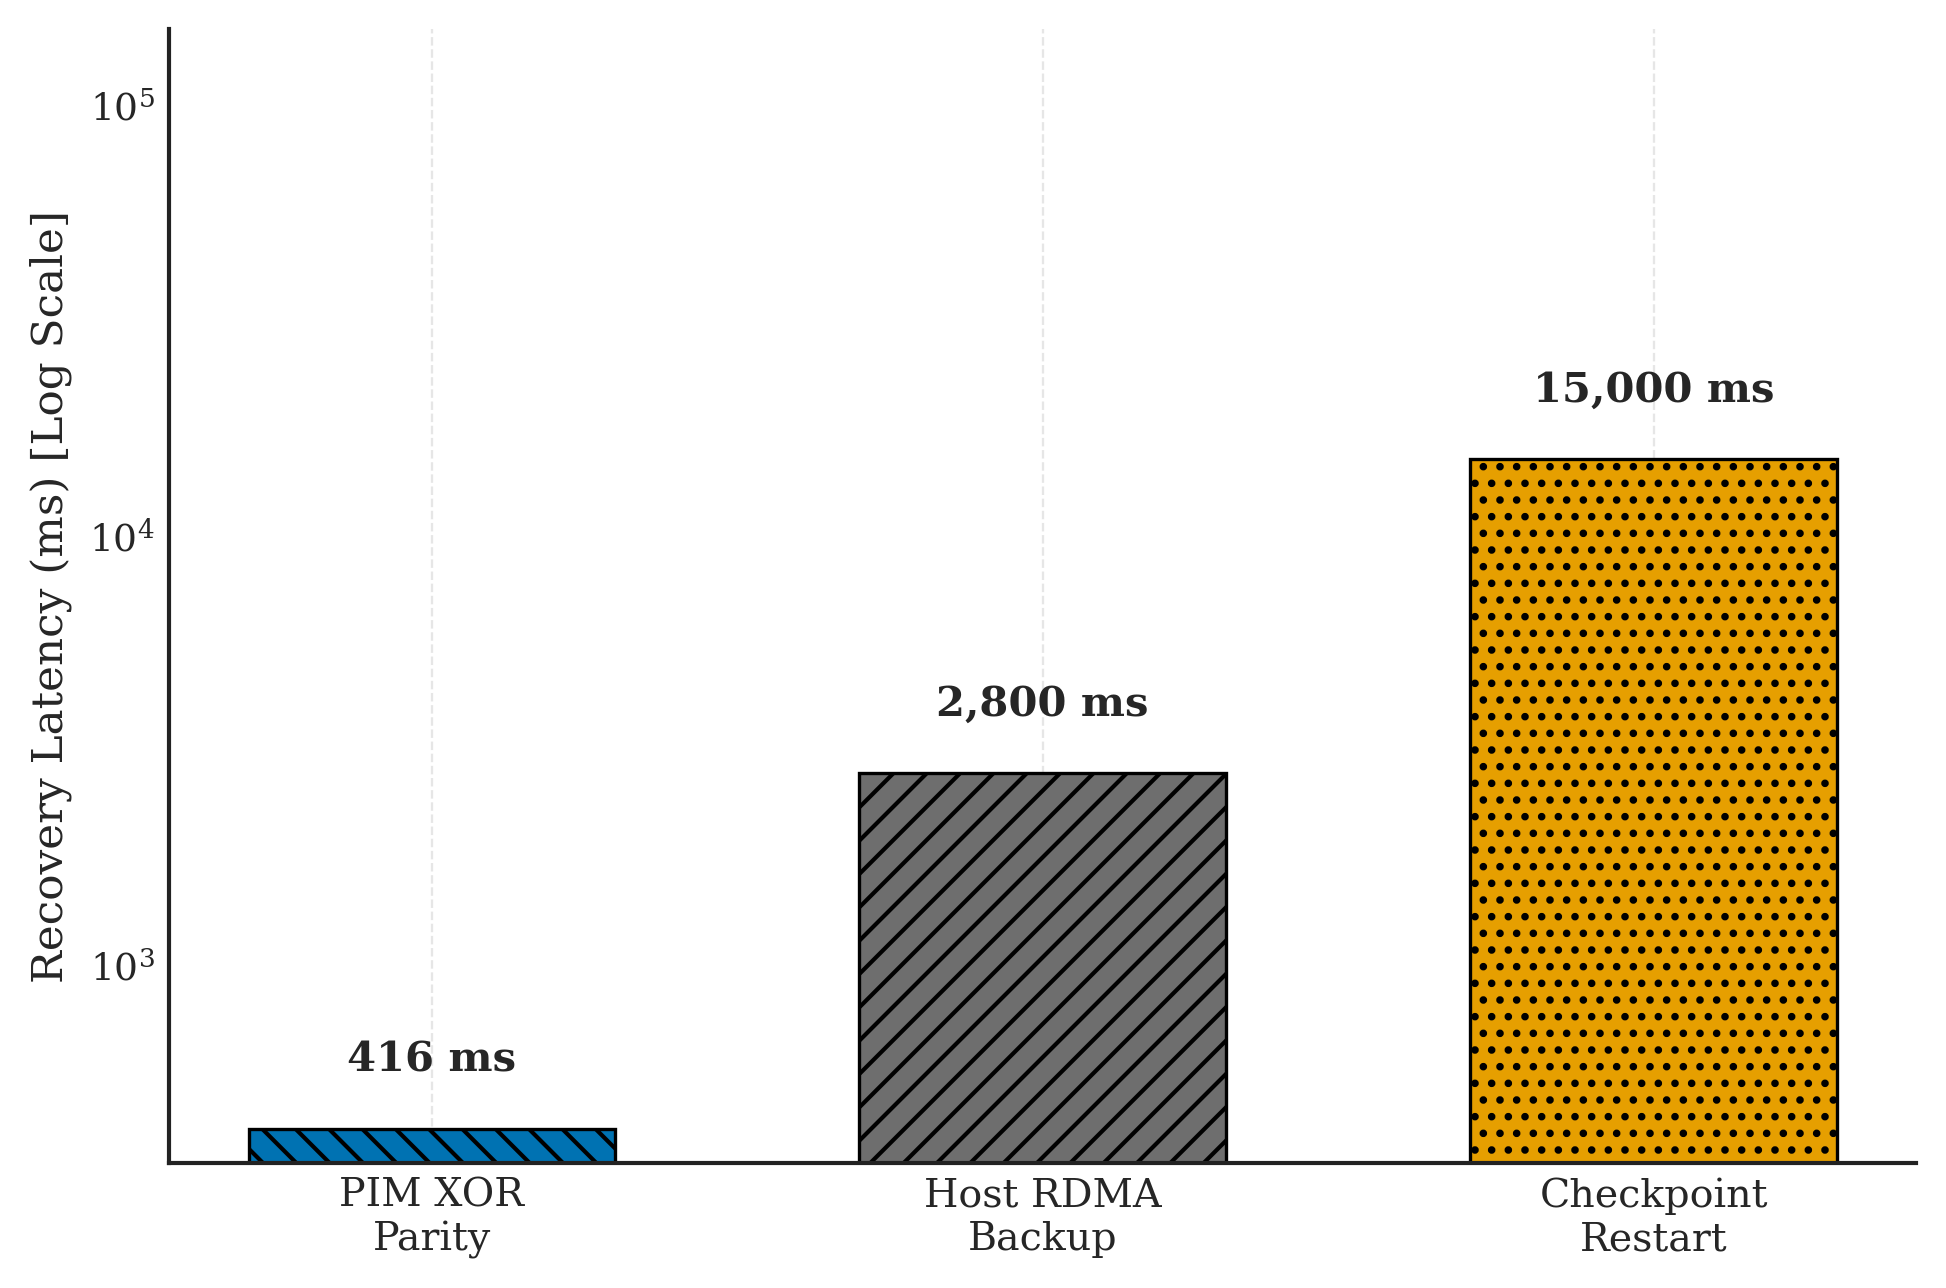
\includegraphics[width=0.78\textwidth]{../paper_assets/figures/fig4_fault_recovery.png}
\caption[Fault-recovery latency comparison]{Recovery-latency distribution for parity-assisted endpoint repair and two host-managed alternatives.}
\label{fig:fault_recovery}
\end{figure}

Figure~\ref{fig:fault_recovery} gives the recovery measurements from the fault-injection artifact. With parity assistance inside DisaggKV, the 95th-percentile recovery time is 416.384\,ms. The two comparison paths are slower by construction: the host-level RDMA backup path is modeled at 2.8\,s, and checkpoint-restart recovery is modeled at 15\,s. The useful point is not only the smaller number; the repair stays close to the endpoint group instead of forcing the host to restart the whole serving path.

The resilience result should be read as localized recovery, not as a complete high-availability design. It shows that short disruption in the endpoint group can be hidden with parity-assisted reconstruction at sub-second timescales in the modeled setting. Persistent device loss, rack-level failures, and request-replay policy require a broader runtime layer than the one evaluated here.
